\learn{3}{}
\section{条件概率}%
\label{sec:条件概率}
\begin{eg}
    有男女生各$50$ 人,有$30$ 个男生和$10$ 个女生抢到了宋浩老师的月饼,求在吃到月饼的学生中男生占比

    分析:总人数$100$ 人为总样本空间$\Omega$,吃到月饼的学生$40$ 人,为第二个样本空间$\Omega_1$

    其中男生有$30$ 人,即概率为:\[
        P\left( A \right) =\frac{30}{40}
    .\] 
\end{eg}
\begin{defi}
    条件概率:$\Omega$ 是样本空间,$A,B$是两个事件,假设$P\left( B \right) >0$ ,求在$B$发生的条件下$A$ 发生的概率,称为$A$ 对$B$的条件概率,记作:
    \[
        P\left( A|B \right) 
    .\] 
\end{defi}
前面提及的概率$P\left( A \right) $ 称作无条件概率,样本空间为$\Omega$ 

条件概率的样本空间发生了变化,$P\left( A|B \right) $ 的样本空间变为了$B=\Omega_B$ 

\subsection{计算}%
\label{sub:计算}
\[
    P\left( A|B \right) =\frac{n_{AB}}{n_B}=\frac{P\left( AB \right) }{P\left( B \right) }
.\] 

图示如下:
\begin{center}
    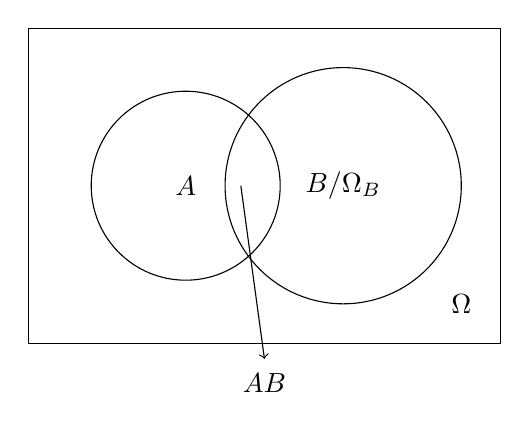
\begin{tikzpicture}
        \draw [] (-3,2) rectangle (3,-2) node at(2.5,-1.5) {$\Omega$};
        \draw [] (-1,0) circle [radius=1.2] node at(-1,0) {$A$};
        \draw [] (1,0) circle [radius=1.5] node at(1,0) {$B/\Omega_B$};
        \node [] () at (0,-2.5) {$AB$};
        \draw [->] (-0.3,0)--(0,-2.2);
    \end{tikzpicture}
\end{center}
\begin{eg}
    有编号$1-6$ 的六个球,随机取一个,观察号码,$B$ 代表号码为偶数,$A_1,A_2$ 代表取到$1,2$ 号,$A_3$ 代表取到大于$4$ ,求:

    1. $$P\left( A_1 \right) =\frac{1}{6}$$

    2. $$P\left( A_1|B \right) =\frac{0}{3}=0$$

    3. $$P\left( A_2 \right) =\frac{1}{6}$$

    4. $$P\left( A_2|B \right) =\frac{1}{3}$$

    5. $$P\left( A_3 \right) =\frac{2}{6}=\frac{1}{3}$$

    6. $$P\left( A_3|B \right) =\frac{1}{3}$$
\end{eg}
\begin{notation}
    条件概率和无条件概率一般不相等
\end{notation}
\subsection{性质}%
\label{sub:条件概率性质}
\begin{rrule}
    \[
        P\left( A|B \right) \ge 0
    .\] 
\end{rrule}
\begin{rrule}
    \[
        P\left( \Omega|B \right) =1
    .\] 
\end{rrule}
\begin{rrule}
    可列可加性:对$A_1,A_2\ldots A_n,\ldots$ 不相容,则:\[
        P\left( \sum_{i=1}^{\infty} A_i | B \right) =\sum_{i=1}^{\infty} P\left( A_i | B \right) 
    .\] 
\end{rrule}
\begin{rrule}
    乘法公式:
    \[
        P\left( AB \right) =P\left( B \right) P\left( A | B \right) =P\left( A \right) P\left( B | A \right) 
    .\] 
    \begin{proof}
        \[
            P\left( A|B \right) =\frac{P\left( AB \right) }{P\left( B \right) }
        .\] 
        \[
            P\left( B|A \right) =\frac{P\left( AB \right) }{P\left( A \right) }
        .\] 
        移项即得上式。
    \end{proof}
\end{rrule}
画图解释如下:
\begin{center}
    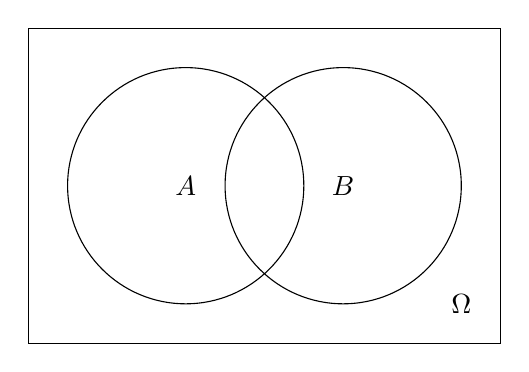
\begin{tikzpicture}
        \draw [] (-3,2) rectangle (3,-2) node at(2.5,-1.5) {$\Omega$};
        \draw [] (-1,0) circle [radius=1.5] node at(-1,0) {$A$};
        \draw [] (1,0) circle [radius=1.5] node at(1,0) {$B$};
    \end{tikzpicture}
\end{center}
